% #############################################################################
% This is Chapter 2
% !TEX root = ../main.tex
% #############################################################################
% Change the Name of the Chapter i the following line
\fancychapter{Problem Definition}
\cleardoublepage
% The following line allows to ref this chapter
\label{chap:problem}

% TODO - ADD PARAGRAPH EXPLAINING SECTION STRUCTURE
This chapter will define the problem, the client requirements and list the necessary functionalities of the solution, to successfully address the problem.
First some context surrounding the problem is given. 
Next, the profile of the target clients will be described, and some examples will be given.
The following section contains a list of client requirements the solution must abide by.
Then it will shed the ligh on some essential concepts in order to understand the operations that need to be implemented.
It will end by detailing those operations.

% -----------------------------------------------------
% -----------------------------------------------------
\section{Context} \label{chap:problem:context}

\begin{figure}[h]
    \centering
    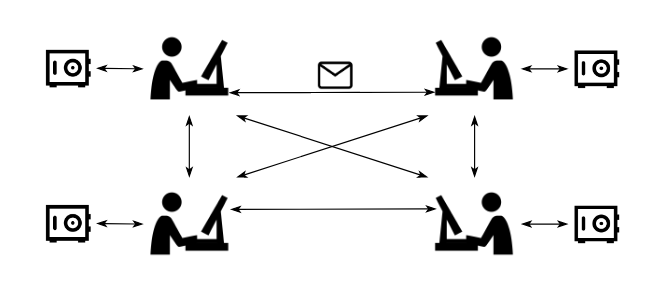
\includegraphics[width=0.5\textwidth]{./Images/main-figure.png}
    \caption{Client communication with their secure devices.}
    \label{fig:main-system}
\end{figure}

As discussed before, the same computers commonly used for communications and information storage are exploitable by attackers, and can cause a minor inconveniences, to possibly severe repercussions, such as, losing your confidential data to malicious parties.

An interesting approach to improve security is to add another layer of security to confidential data and communications through the addition of an device, independent of the user's personal computer. The device is responsible for the security of sensitive data and communications.

An illustration of the system with multiple users can be seen in figure \ref{fig:main-system}.

\subsection{Entities} \label{chap:problem:entities}

These type of devices are especially relevant to people high responsibility jobs, that handle very sensitive information, which have dire consequences if they are lost, corrupted or leaked.
Some examples are government officials who handle confidential information pertaining to a country, company executives, such as the CEO who have access to company secrets, diplomats who manage confidential treaties, and military officers who have access to information critical to a countries' security.

% Talk about groups and individuals
Additionally, not just individuals have interest in these systems, a device can be assigned to a group of people representing an entity. For example, in the armed forces, a device can be assigned to the navy, one to the infantry, and every other faction. Any ranked officer, or people with a certain level of authority, could use the entity device, to communicate with other people or entities, in behalf of the group.

\subsection{Devices} \label{chap:problem:devices}
% Devices
There are currently on the market some dedicated devices designed to secure communications and save private data.
These type of devices have physical tamper-resistant measures against attackers who wish to read the device's information. They also provide fail-safe mechanisms in case of an attack.
Hardware Security Modules (HSM) are high grade devices, with more computational power and larger storage capacity for the user's secrets.

Smart Cards, provide secure and portable tamper-resistant storage.
They have lower processing power, and smaller memory which only allows to store a small amount of data.
They have a low-cost, so can be produced in bulk and easily replaced. Only an RFID card reader is needed to read its information, and verify the owner's identity.
Because of these features, they are widely used in the retail, healthcare, communication and government industries.


% -----------------------------------------------------
% -----------------------------------------------------
\section{Client Requirements} \label{chap:problem:requirements}

% TODO - more high level

To effectively address the presented problem, there are several high-level requirements the solution must adhere to:
\begin{itemize}
	\item Devices should be distributable to either individuals, entities composed of multiple people or groups of people;
	\item The system must allow communications between groups of people and individuals representing themselves or an entity;
	\item The system must be responsible for securing all communications against disclosure, tampering or any sort of attacks;
	\item The device should be dependent from user's personal computers. This way, the user's do not need to worry about what computer they use, the device is responsible for providing all the functionality;
	\item Users should be able to choose who they want to initiate secure communications. The application should provide the functionality to allow this;
	\item Is should be simple to use by everyone, including non-technical people;
	\item It should have a relatively low cost, enough to allow distribution of several devices between multiple individuals and groups;
	\item Only individuals with a certain level of clearance should be authorized to use the device. Personal devices should only be accessible by their owners.
\end{itemize}

% -----------------------------------------------------
% -----------------------------------------------------
\section{Concepts} \label{chap:problem:concepts}

In this section some necessary concepts will be explained in order for non-technical users can easily understand the background, as well as the necessary concepts to fulfill the previously defined requirements.

Some services are crucial, in order to guarantee the security of communications.

\textbf{Confidentiality} is a security service which keeps the contents of communications secret, except from the authorized parties.

\textbf{Integrity} safeguards communications from modifications by attackers.

The \textbf{authentication} service can verify the identity of an agent, taking part in the communications.

Finally the \textbf{non-repudiation} service prevents an entity from denying authorship of a piece of information.

\textbf{Cryptographic keys} are tools used to grant the aforementioned services. Users in possession of the keys can secure and access their messages.

\textbf{Symmetric keys}, in possession of all communicating parties, are used to secure messages and documents.

\textbf{Asymmetric key pairs} (public and private key), are used to enable communicating by for example, sharing new symmetric keys between users who wish to communicate. Secondly, they provide non-repudiation through digital signatures.
These keys identify the owner. The private key must always be in possession of the owner. With it they can prove their identity and generate signatures.
The public key should be shared with other people so that they can share keys and verify the owner's signatures.

\textbf{Digital signatures} are a digital version of handwritten signatures, commonly used anywhere forgery detection is essential, for instance in financial transactions.
Qualified signatures are a special type of signatures where the private keys are generated and stored inside a device, such as a Smart Card, and never leave it.
This strong signature legally represents a person or a group. This type of signatures are used in the Portuguese Citizen Card.

% -----------------------------------------------------
% -----------------------------------------------------
\section{Solution Services} \label{chap:problem:services}

% TODO - more high level
% groups and keys

This section will go into more technical detail on the services the solution should provide taking account the client requirements and the essential concepts.

\subsection{communications} \label{chap:problem:services:comms}
In order to secure communications, the following services must be guaranteed: confidentiality, integrity and authentication.
The system must also give an option to provide non-repudiation to documents or files, by means of digital signatures.


\subsection{Key management} \label{chap:problem:services:key}
The device must store all the symmetric and asymmetric keys related to the entity or individual who owns the device.

The device must support secure storage in order to store the user's sensitive information, such as the cryptographic keys used for communication.
Additionally, the device should have physical tamper-resistant measures and mechanisms in place, in case of an intrusion, such as, permanent erasure of all sensitive data. 
This means that even if an attacker is in possession of the physical device, it should be extremely difficult or even impossible to extract any information from it.

These keys must never be exposed to the outside environment of the device to ensure the security of communications and independence of the system.

All cryptographic operations must also be performed inside the device.

Key management operations should be supported, namely: symmetric key generation, symmetric key revocation, if communications are suspected to be compromised, and importation of other user's public keys.

Each entity has one pair of asymmetric keys, stored in their device, a private and a public. This pair identifies the entity.
For each channel of communication between individual users, groups or entities, the same symmetric key is stored in both devices.

When a new user wants to establish secure communications with an existing user or a group, he must share his public key with the user, ideally physically to ensure there are no mistakes or attacks. After this they can securely share symmetric keys, and establish a new secure communication channel when the keys are stored in their devices.

The users will receive the device with a pair of asymmetric keys, a private and public, generated inside the device from fabric. Each device will have the user's public keys, whom he wishes to communicate. The user can request whose public keys he wants, before the device is initialized in fabric. This allows the users to share symmetric keys between them, which they can user to begin trading data securely. The device can also come with the symmetric keys already shared and stored in each user device.

\textbf{Public-Key Cryptography Standards (PKCS) \#11} are a group of widely used cryptographic standards, which define an application programmable interface (API) designed to manipulate common cryptographic objects, such as keys.
With this API, the objects can be used, created and modified by applications, without exposing them to the application's memory.
The solution should follow this standards, to increase its independence and security requirements.

% --- authentication ----
\subsection{Authentication} \label{chap:problem:services:auth}
Every user must authenticate himself, before using the device. This is done by providing a PIN code, which the device will verify before unlocking the session for the user.

The device will come from fabric with a default authentication PIN. This code can be changed by the users.

For personal devices, there is only the owner, but for groups and entities, there can be multiple users. In this case, there are two different ways to authenticate. The simplest is not to authenticate the person using the device, but have a single authentication PIN for the entity. All the user's with permission to communicate in behalf of the entity, must know the PIN code.

The second option, is to authenticate the user itself. The advantage of this approach is there can be a log of which users used the device and when, and what messages were sent and received for each user.
This would entail a more complex process where, each user allowed to use the device, must register with a name and individual PIN code. The initial PIN code, would be used as an administration code, which allows registering users, and accessing the logs of user operations and message transactions.

It is worth nothing only the users are authenticated, the device does not authenticate itself to the user.

\subsection{Usability} \label{chap:problem:services:usability}
There are also several usability requirements the solution must abide by.

\subsubsection{Device Standardization}

The solution should work with a plethora of devices, which will increase the adoptability of the solution among clients. This entails the use of a widely established protocol, which clearly defines a set of functions and standards the system should follow.
This is where the PKCS \#11 standard is again relevant. By implementing the system in accordance with these guidelines, it will have a higher device interoperability.

\subsubsection{Client Application}

The system should provide an application on the user's device, which will communicate with the physical device, and make the operation's available to the user through a simple interface for the regular non-tech savvy user.
Since the goal is a simple application which interfaces with the device, there is no need for a specific and specialized tool to run the application. It should ideally be available by default in the most popular workstation operation systems, e.g. Windows, MacOS and Linux. This will simplify the system's setup operation.

Another related requirement is the usage of a common connection solution, e.g. USB cable, to further increase the pool of supported devices.

In addition, the system should perform the operations in a reasonable time to minimize the user's wait, and improve the user experience.
